\graphicspath{{chapters/04/images/}}
\chapter{Damage response}

\section{Introduction}
Biocompatibility is the ability of a material to perform with an appropriate host response in a specific application.
The first system interacting with the scaffold is the immune system, which first gives an immuno response and then starts the healing process.
The immune system is tissue specific and changes based on the pathogenic status of it.
The loss of regenerative capacity of an individual throughout its lifespan is linked to the evolution of immune competence.
Taking for example a wound of the skin, in a fetus complete regeneration without scar tissue formation can be observed, whereas in adults fibrotic healing takes place.
Some parameters from the fetal models can be taken into account when designing a scaffold that will reduce the formation of scar tissue in adult patients.
The relationship between tissue healing and the immune response is very complex: factors can have both a positive or negative effect, depending on the tissue and the organ involved in the injury and the life stage (that can be embryonic, neonatal or adult) of the patient.
In order to prioritize healing, the inflammation must be reduced as soon as possible.

\section{Tissue damage}
A damage to the tissue will cause bleeding, the accumulation of pathogens and cell debris at the site of the open wound.
After a tissue suffers a damage, the immune system gets activated and recruited to the damage location, causing an inflammatory response.
This inflammatory response is a defense step and it can be divided in sub-steps:

\begin{multicols}{2}
	\begin{enumerate}
		\item Platelet activation.
		\item Coagulation cascade.
		\item Inflammation.
	\end{enumerate}
\end{multicols}

After these steps the system will be activated for regeneration.

	\subsection{Timeline of tissue regeneration}
	In 3-7 days cell begins to migrate and proliferate in the wound site, promoting ECM and other molecule's synthesis and angiogenesis.
	External pathogens are dealt by scar tissue formation, blocking the entrance of the wound, while internal pathogens are dealt by inflammation increasing the blood flow into the damaged site through angiogenesis.
	This overall process is controlled by the inflammatory system cells like macrophages coordinated by interleukines (IL-1 and IL-2).
	During this time period (processes visualized in \ref{fig:roles}):

	\begin{multicols}{2}
		\begin{itemize}
			\item Free particles like cell debris or other external factors are opsonized with c3b antibodies for phagocytosis.
				This is done so that macrophages can recognize pathogens through the attached integrins.
			\item The inflammatory reaction is elicited through factors acting on leukocytes, mast cells and endothelium.
			\item At the end complement-mediated cytolysis happens, destroying the pathogens.
		\end{itemize}
	\end{multicols}

	\begin{figure}[ht]
		\centering
		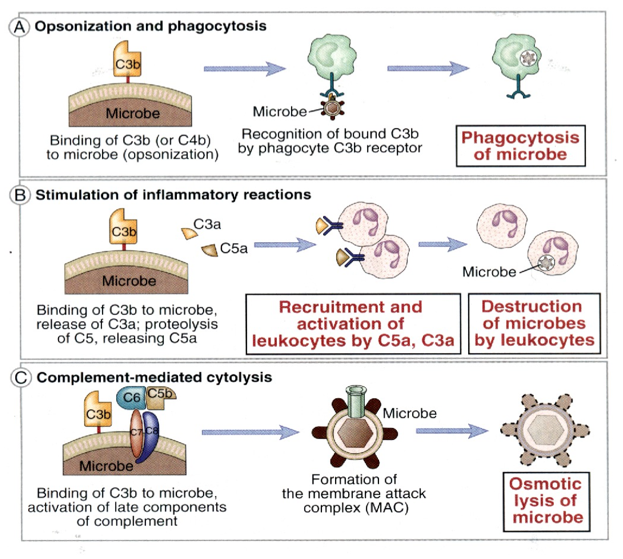
\includegraphics[width=\textwidth]{roles}
		\caption{\label{fig:roles}}
	\end{figure}


	\subsection{Immune system response}

		\subsubsection{Inflammatory response}
		The inflammatory response is the body’s natural response that occurs immediately following tissue damage.
		Its main functions are to defend the body against harmful substances and to promote the renewal of normal tissue.
		Signs of inflammation include:

		\begin{multicols}{2}
			\begin{enumerate}
				\item Pain due to chemical released by damaged cells.
				\item Swelling or edema due to an influx of fluid into the damaged region.
				\item Redness due to vasodilatation (widening of blood vessels and bleeding in joint or structure).
				\item Heat due to an increase in blood flow to the area.
				\item Loss of function due to increased swelling and pain.
			\end{enumerate}
		\end{multicols}

		The inflammatory reaction is the combination of a number of overlapping reactions within the body.
		Although a lot of these occur simultaneously, a certain order of events may be seen.
		The tissue damage may occur from trauma such as a tackle, collision or from a fall.
		However, quite commonly tissue injury is as a result of overuse (microtrauma) or pathology.
		So, when tissue cells become injured, a number of chemical like kinins, prostaglandin and histamine are released to initiate the inflammatory response.
		These chemicals work collectively to increase vasodilation (widening of blood capillaries) and the permeability of capillaries.
		This leads to increased blood flow to the injured site.
		These substances also act as chemical messengers that attract some of the body’s natural defence cells through chemotaxis.
		Although highly beneficial to the body’s defence strategies, some chemicals also increase the sensitivity of the pain fibres in the area and so the area becomes painful.

		\subsubsection{Immune system population}
		The immune system involved in response to a wound is composed by leukocytes, which can be further divided into neutrophils and monocytes.

			\paragraph{Neutrophils}
			Neutrophils or polymorphonucelar are the most abundant circulating leukocytes.
			They are two types of intracellular granules, which are common progenitors for monocytes.
			Our body produces around $10^{11}$ per day, with a $6$ hours lifespan, before apoptosis.

			\paragraph{Monocytes}
			Monocytes and activated macrophages are phylogenetically the oldest cells in the immune system.
			They circulate as inactive monocytes, and become activated macrophages when they enter a damaged tissue.
			They are typically located in:

			\begin{multicols}{2}
				\begin{itemize}
					\item The subepithelial connective tissue.
					\item The interstitia of parenchymal organs.
					\item The lining of vascular sinusoids in liver and spleen.
					\item The lymphatic sinuses of lymph nodes.
				\end{itemize}
			\end{multicols}

			They usually respond later than neutrophils at sites of injury and infection and they are the primary effectors of the innate immune system.
			The primary purpose of these phagocytes is to clear the wound from invading organism, everything that is non-self material.
			They can exist for years.

		\subsubsection{Phagocyte-mediated wound cleaning}
		Phagocyte-mediated wound cleaning is used to produce new vessels from new cells and it consists of different passages:

		\begin{multicols}{2}
			\begin{enumerate}
				\item Recruitment: adhesion proteins facilitate attachment to endothelium.
				\item Migration: receptors that mediate chemotaxis to target site.
				\item Recognition and phagocytosis: specific receptors for microbes and opsonized materials driving phagocytosis.
					Fc receptors and C3 receptors are major mediators of the attachment.
				\item Release of cytotoxic compounds: reactive oxygen and nitrogen species.
				\item Cytokine production and secretion of numerous cytokines and chemokines with local and systemic activity:
					 \begin{itemize}
						\item Positive factors: increase macrophage activation, recruitment and  stimulation of the adaptive immune system.
						\item Negative factors: inhibit activation and proliferation of the immune system.
						\item Secretion of factors that facilitate wound remodelling, matrix production and angiogenesis.
					\end{itemize}
			\end{enumerate}
		\end{multicols}

			Macrophages dominate biomaterial interfaces in tissues and are often present chronically.
			There is a need to control the interaction of the scaffold with macrophages to avoid pro inflammatory signals.

		\subsubsection{Leukocyte extravasation}
		Leukocytes in physiological condition travel through the blood capillaries.
		When a tissue is damaged a chemotactic signal is sent to them through molecules like bacterial peptides causing their adherence to endothelial cells.
		Then integrins and I-CAM binds them causing adhesion and process formation, with additional signals and ligands promoting migration.
		The overall process is described in figure \ref{fig:leuko}.

		\begin{figure}[ht]
			\centering
			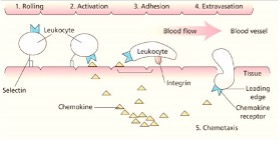
\includegraphics[width=0.4\textwidth]{leuko}
			\caption{\label{fig:leuko}}
		\end{figure}

		\subsubsection{TNF-$\alpha$}
		TNF-$\alpha$ is the principal mediator of acute inflammation.
		It is produced by macrophages and activates the pro-inflammation NFkB transcription factor.
		Doing so, it increases the endothelial expression of selectins and integrins, production of chemokines in endothelial cells and macrophages and the production of prostaglandins and leukotrienes like pyrogens and chemotactic.
		It also induces prostacyclin expression in the endothelium, increasing local blood flow and production of IL-1 in macrophages.

		\subsubsection{Leucokytes migration}
		All of this signals cause chemotaxis of macrophages and neutrophils to the damaged area.
		Neutrophils are the first to reach the injured site and neutralize harmful bacteria.
		Macrophages aid the healing process by engulfing bacteria and dead cells and ingesting them, clearing the area and creating a favourable environment for new cells to grow.
		They can be found at the injured site within the first $72$ hours and remain in it for weeks.

		\subsubsection{Major activities of macrophages secreted factors}
		The inflammatory system, with the aim of reaching healing, goes through scar tissue formation, its modification and then regeneration.
		Macrophages react to inflammation by killing microbes and phagocyting them, guided by oxotin produced by the system.
		The passage through scar tissue is necessary to defend the system from pathogens.
		So regeneration will happen only at a later stage.

		\subsubsection{Inflammatory monocytes}

		\begin{figure}[ht]
			\centering
			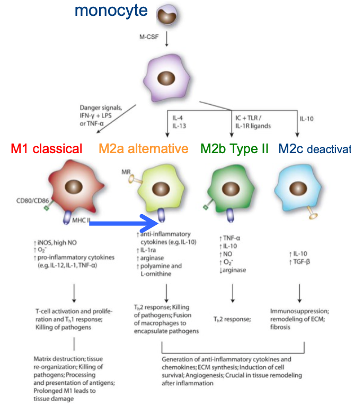
\includegraphics[width=0.4\textwidth]{mono_diff}
			\caption{Monocytes differentiation process}
			\label{fig:mono}
		\end{figure}

		Figure \ref{fig:mono} depicts macrophages differentiation from classical proinflammatory to regenerative.
		Each one is characterized by a specific profile of released molecule, which can be used to identify them.
		This identification is useful to see the interaction between the scaffold and the inflammatory cells and see if they are able to produce angiogenic and regenerative factors.

		\subsubsection{Inflammatory cellular response}
		Opsonin allows the macrophages to recognize and digest a foreign body like cancer cells.
		This process involves moving it inside the cellular membrane of the macrophages.
		When a scaffold is introduced into the injury site cells respond with:

		\begin{multicols}{3}
			\begin{itemize}
				\item Oxidative burst.
				\item Bacterial killing.
				\item Tissue injury.
			\end{itemize}
		\end{multicols}

		If the material is very sensitive, it will release some fragments that will be destroyed by macrophages and will cause necrosis in the surrounding tissue.
		Doing so, this particles will upregulate the inflammatory response, causing its transformation from acute to chronic.
		When designing a scaffold the aim is to reduce as much as possible the intensity and time of this response and, in doing so, the formation of scar tissue.

		\begin{figure}[ht]
			\centering
			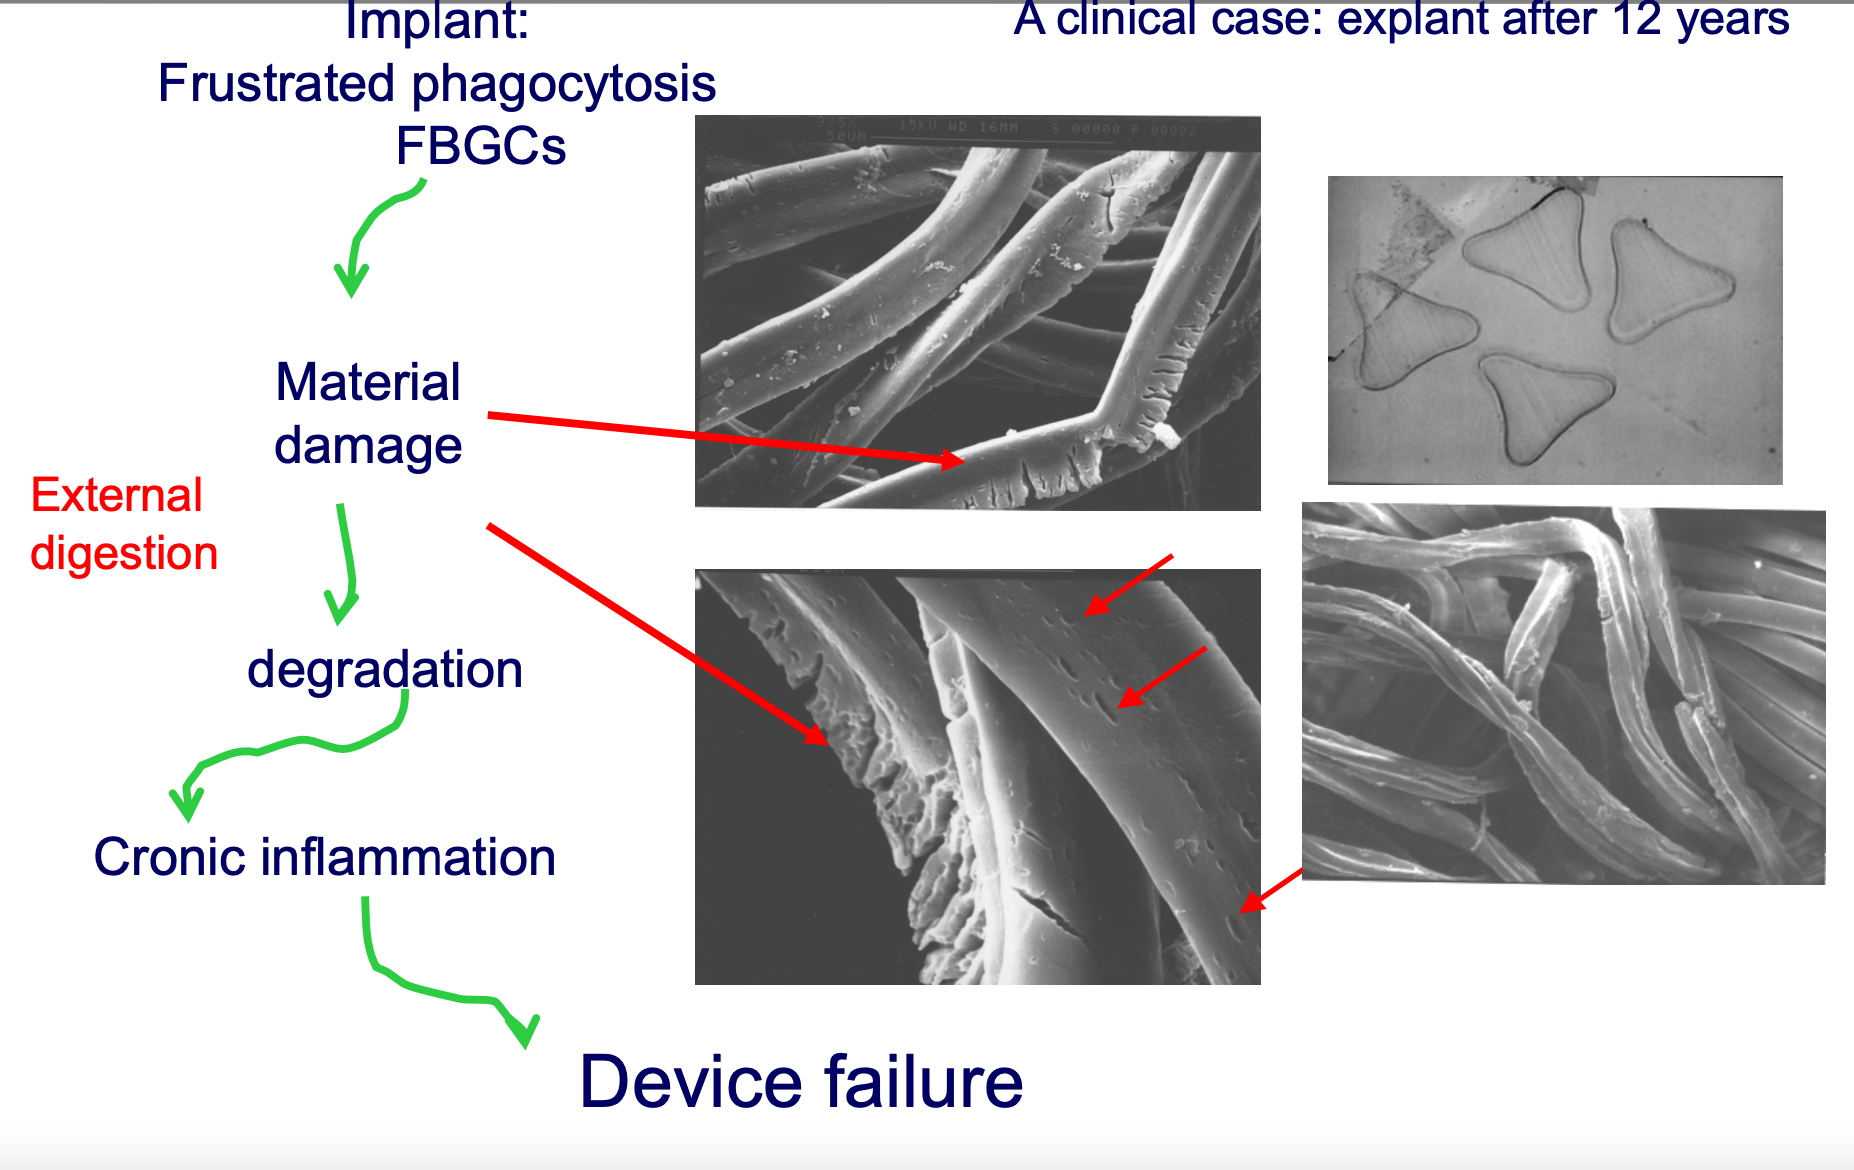
\includegraphics[width=0.6\textwidth]{failure}
			\caption{\label{fig:failure}}
		\end{figure}

		Figure \ref{fig:failure} shows the interaction between cells and material in an implant, explanted after 12 years due to failure.
		The tube changed its shape and diameter, provoking blood turbulence, and increasing thrombosis risk.
		The problem with this implant is that space was occupied by macrophages, which were able to adhere and digest the external fibers, causing their release in the form of microparticles.
		The prosthesis was made in nylon, a really stable polymer.
		Since it is stable and strong, the human body sensed it as foreign and started damaging it.
		The section of the damaged fibers was triangular.
		This continuous digestion process caused chronic inflammation, and, in the end, failure of the implant.

	\subsection{Wound healing in skin}
	After damage of the skin, the regeneration process begins.
	This consists of:

	\begin{multicols}{2}
		\begin{enumerate}
			\item Acute inflammation.
			\item Proliferation.
			\item Remodelling.
			\item Restoring of the tensile strength.
		\end{enumerate}
	\end{multicols}

	The synthesis of collagen occurs between 7 and 14 days.
	After 14 to 21 days, collagen cross-linking assembling begins.
	During this process collagen has less cross-links, so it is more flexible but less strong.
	The immune system must be controlled as to induce tissue regeneration.

		\subsubsection{Macrophage transition}
		Right after the injury pro-inflammatory macrophages, phagocytes of type $I$ will produce cytokines.
		When they remove all the debris, type $I$ macrophages differentiate into type $II$ macrophages, leading to the downregulation of pro-inflammatory cytokines and tissue regeneration.
		When designing a scaffold this transition from type $I$ to type $II$ has to be carefully planned to shift from an acute inflammation to regeneration.

		\subsubsection{Main actors of the immune response}
		The main actors of the immune response following tissue injury are:

		\begin{multicols}{2}
			\begin{itemize}
				\item Kinetic of immune cell mobilisation after tissue injury.
				\item Initial inflammatory phase following tissue injury.
				\item Immune mechanisms that can impair tissue healing or drive to scarring and fibrosis.
				\item Pro regenerative immune mechanisms.
			\end{itemize}
		\end{multicols}

		\begin{figure}[ht]
			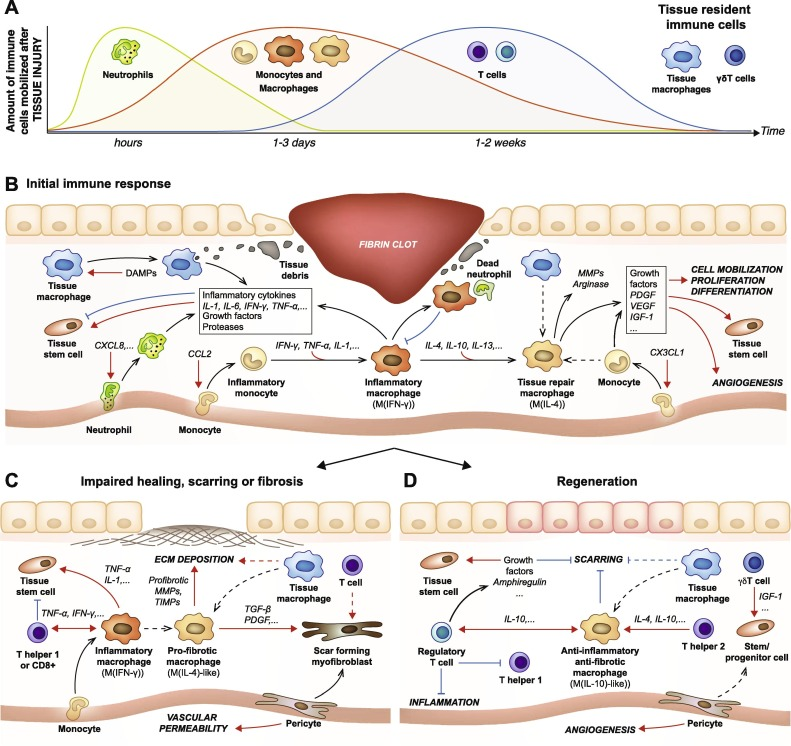
\includegraphics[width=1\textwidth]{healing}
			\caption{\label{fig:healing}}
		\end{figure}

\section{Tissue healing}
The process of tissue healing can be divided into four parts:

\begin{multicols}{2}
	\begin{enumerate}
		\item Collagenation and cartilarisation.
		\item Angiogenesis.
		\item Proliferation.
		\item Remodelling.
	\end{enumerate}
\end{multicols}

	\subsection{Revascularization}
	Revascularization happens when the damaged area begins to sprout new capillaries to bring  blood to the regions once sufficient cleaning has been achieved.
	The new capillaries must sprout in an ordered manner, which must be taken into account during scaffold design.
	When blood flow has been re-introduced to the area, specific tissue cells begin to re-grow.
	For example, in a muscle tear muscle cells will repopulate the area.
	Wound healing occurs towards the end of the inflammatory process, however the two processes overlap considerably.

	\subsection{Collagenation}
	Macrophages work to clear the damaged area and make space for the regeneration of the new tissue.
	After a number of days, fibroblasts (collagen producing cells) begin to construct a new collagen matrix, which will act as the framework for new tissue cells.
	Tissue healing occurs with the sprout of new capillaries to bring blood to the region (revascularization).
	A path for interconnection must be built by playing with scaffold architecture and the release of angiogenetic factors.

	\subsection{Proliferation}
	The proliferation phase lasts 4 weeks.
	In cases where the injury has been more severe, the affected area may be composed by a mixture between specific tissue cells (such as muscle cells) and other tissue known as granulation tissue.
	If this granulation tissue is not removed it will remain and form scar tissue, which can lead to a decreased functional ability of the tissue.

	\subsection{Remodelling}
	Remodelling occurs when new cells mold into their surrounding to once again produce a functional tissue.
	This process can take months or even years, altering the new tissue slowly.
	The new cells and protein fibers become arranged in a way that is best suited to the stresses imposed on the tissue.
	Hence, when a tissue is healing, it is important to stretch it in the correct direction, so as to optimise the strength of the new tissue.

	\subsection{Strategies to promote tissue regeneration}
	There are different strategies based on biomaterials and drug delivery systems to promote tissue regeneration by controlling the immune system:

	\begin{multicols}{2}
		\begin{itemize}
			\item Physicochemical properties of the scaffold.
				Degradability, hydrophobicity and topography must be kept in mind.
			\item Pro-inflammatory modulators.
			\item Anti-inflammatory modulators.
		\end{itemize}
	\end{multicols}

	Materials must be chosen according to:

	\begin{multicols}{2}
		\begin{itemize}
			\item Protein adsorption.
			\item Generalised toxic effect.
			\item Inflammatory cell activation.
			\item Fibrosis.
			\item Microvascular changes.
			\item Tissue-organ specific cell response.
		\end{itemize}
	\end{multicols}

	The scaffold must activate or inhibit specific pathway, depending on the injury and on the tissue.
	These can be:

	\begin{multicols}{2}
		\begin{itemize}
			\item Activation of clotting cascade.
			\item Platelets adhesion, activation and aggregation.
			\item Complement activation.
			\item Antibody production.
			\item Immune cells response.
			\item Hypersensitivity.
			\item Mutagenesis, genotoxicity.
			\item Tumour formation.
		\end{itemize}
	\end{multicols}

	Everything is controlled by the material, the environment and their interaction.
	When the biomaterial is recognized as a foreign body, macrophages are recruited and cells will not be able to migrate on the scaffold for regeneration, resulting in a complete failure.

		\subsubsection{Effects oh physiochemical modification to biomimetic scaffolds in musculoskeletal applications}

		\begin{figure}[ht]
			\centering
			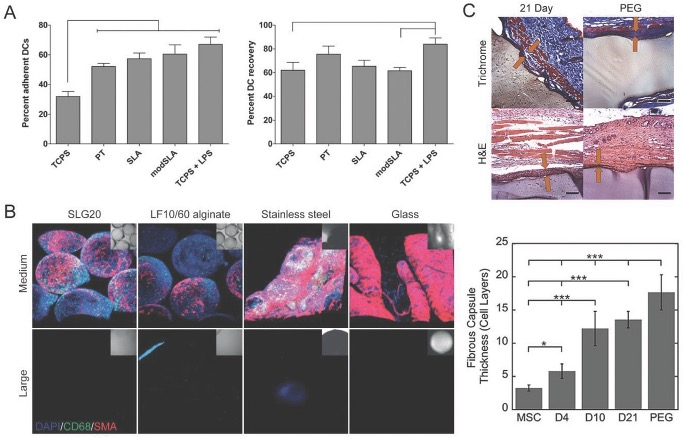
\includegraphics[width=0.5\textwidth]{muscosk}
			\caption{\label{fig:muscosk}}
		\end{figure}

		In figure \ref{fig:muscosk} the percentage of dendritic cells (inflammatory cells) in the sample can be identified.
		A different adhesion degree of inflammatory cells to the scaffold can be obtained changing the physical characteristics of the scaffold or the molecules with which it is functionalized.
		In panel B the different shape and thickness for each material can be seen.
		Moreover the control of dendritic cells' phenotype from pro-inflammatory to toleragenic is of interest during scaffold design.
		Their phenotype is modulated by the innate immune cell types.

		\subsubsection{Processes that affect the biological outcome}
		The capability of a scaffold to absorb protein is important as it can cause an inflammatory response.
		In fact different protein conformation can control the water content, reducing it by increasing cristallinity, leading to different mechanical properties.
		It can be noted how a small amount of proteins is still able to induce a high pro-inflammatory reaction.

		\subsubsection{Empowerment of stem cells by inflammation}
		Immune cells at the site of tissue injury, including macrophages and T cells, secrete TNFalpha, TNFy, IL-1, IL-13 and other pro-inflammatory cytokines, which in turn can activate stem cells.
		Once licensed by these cytokines, stem cells can facilitate tissue regeneration though cell differentiation and the release of anti-inflammatory cytokines and growth factors.

		\subsubsection{Designing immuno informed biomaterials matrices}
		When designing a functionalized scaffold a level of safety should be provided, non including tumorigenetic factors.
		The molecules need to functionalize the scaffold can be delivered through extracellular vesicles.
		The topography and the chemistry of the scaffold play a central role in this process as macrophage polarization and network formation.
		The network should be formed in 3D on the surface, providing interconnections for macrophages.
		For instance, after scaffold implantation protein adsorption is observed, followed by macrophages adherence that cause the formation a network speeding up the process toward regeneration.
		Macrophages are also involved in vascularization.
		When the scaffold is not porous the macrophages will not be able to polarize and switch to state $II$, inducing the formation of scar tissue.

		\subsubsection{Effect of topography and stiffness on macrophages polarisation}
		Macrophages assume an elongated shape when switching to the M2 like phenotype with an up-regulated expression of arginase, on PDMS substrates with 2 gratings topography compared to planar control.
		After the adhesion (f), cells start to polarize (g) [figure \ref{fig:topo}].
		Increased stiffness in hydrogel drives the transition in absence of cytokines stimulation.

		\begin{figure}[ht]
			\centering
			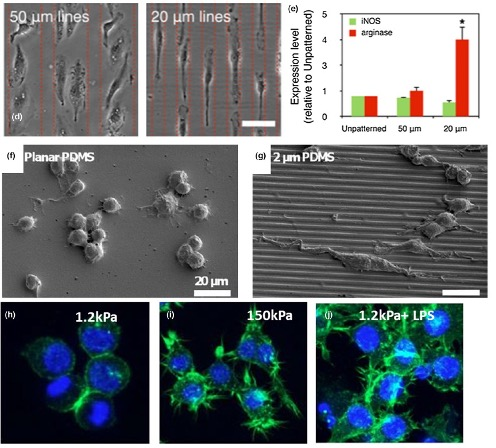
\includegraphics[width=0.5\textwidth]{topo}
			\caption{Macrophages and scaffold topography\label{fig:topo}}
		\end{figure}

		\subsubsection{Role of pore size, distribution and degradation}

		\begin{figure}[ht]
			\centering
			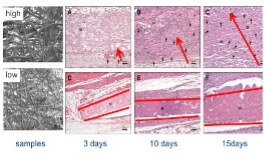
\includegraphics[width=0.4\textwidth]{silk}
			\caption{\label{fig:silk}Silk fibroin micro-nets formic acid treated: In vivo evaluations}
		\end{figure}

		Figure \ref{fig:silk} depicts silk fibroin micro-nets formic acid treated in an in vivo evaluation.
		In this case we have induced regeneration in unnatural conditions.
		Changing the pore size, the mechanical properties will be affected.
		In high porosity samples after 3 days we have granulated tissue (dots are cells), the scaffold was able to promote movement inside.
		At 10 days the arrows are indicating new capillaries.
		Macrophages are at phase II, cells have more space to build tissue.
		Then thinner fibers, blood vessels, not so many dots, signalling that inflammatory cells almost disappeared.
		Already after 3 days we have a very clear scar tissue formation, which becomes thinner in 10 days.
		We have also different vascularisation and degradation depending on porosity.

		\subsubsection{Regeneration of non-vascularized tissues}
		Since the mechanism of inflammation depends on the blood, non-vascularized tissues are generally hard to regenerate.
		When designing a scaffold different approaches are needed in these cases.
		An example is a damage to the cartilage-bone interface.
		The first is a soft, unnerved and non vascularized tissue, while the second one is a robust, innervated and vascularized one.
		In this situation we need a gradient-rich scaffold that allows for correct tissue and interface regeneration, while avoiding blood vessel formation in cartilage that would drive the inflammation in the latter and transform it into bone.
		We can trap vessels in the bone section by playing with porosity, and we could tackle the cartilage section regeneration using injectable biocompatible gels filled with the appropriate cells.

	\subsection{Possible outcomes after the inflammatory response}
	After the intervention of macrophages and neutrophils and the death of neutrophils the immune system could face three different situations.

		\subsubsection{Clear situation}
		If the situation is clear: there is no more damage or pathogen that can be detected by immune cells and the remaining damage is of moderate extension.
		Local adaptive and innate immune cells produce anti-inflammatory cytokines IL-4, IL-10, IL-13 and TGF$\beta$ leading to the definition of a resolving environment that leads to macrophage polarization towards the M2 phenotype.
		This macrophages appear elongated and rich in protrusions.
		This phenotype communicates with local stem cells, mobilizing them and causing their proliferation and differentiation, and with local firbroblasts, triggering scar-tissue remodelling.
		In this process the temporary matrix is digested and a tissue specific ECM is deposited, leading to healing by regeneration.
		This remodelling process can take months or even years.

		\subsubsection{Clear situation with extensive damage}
		If the situation is clear but the damage is too extensive: while the removal of the harmful stimulus leads to the release of anti-inflammatory cytokines and to the polarization of M1 (inflammatory and microbidical) macrophages into M2 (immunomodulatory and reparative), and while these are successful into driving the local fibroblasts into a tissue remodelling status, the abundance of the scar tissue itself is a limit to the enzymes’ proficiency: the scar tissue will remain, impacting the mechanical and functional characteristics of the tissue.

		\subsubsection{Not clear situation}
		If the situation cannot be cleared, after an appropriate period of time, usually one or two weeks, lymphocytes and plasma cells join M1 macrophages in a context characterized by cyclical instances of tissue healing by repair and tissue damage by immune cells’ oxidizing activity.
		M1 macrophages are the vast majority, since the situation does not allow for the production of the anti-inflammatory cytokines needed for M2 polarization.
		There is the fusion of macrophages to form giant cells, which recruit fibroblasts causing excessive collagen deposition and formation of fibrous scaffolds and scar tissue.
